%%%%%%%%%%%%%%%%%%%%%%%%%%%%%%%%%%%%%%
\section{数値解析法}
\subsection{FDTD法}
前節で示した方程式に離散化に,FDTD(Finite Difference Time-Domain)法を用いる.
時間ステップ長を$\Delta t$, スタガード格子の$x_i$軸方向の間隔を
$\Delta x_i,(i=1,2)$とし,その間隔は一定とする.この間隔で時空間内に配置された差分格子における関数$f(\fat{x},t)$の値を$f^k_{i,j}$と書くことにする.ただし,$k$は時間ステップを,$i,\, j$は$x_1$および$x_2$方向の格子位置を表す番号を意味する.このとき,中央差分で時間微分を近似すれば,
\begin{equation}
	\dot{f}^{k+\frac{1}{2}} \approx \frac{ (f)^{k+1}-(f)^k}{\Delta t}
	\label{eqn:dfdt}
\end{equation}
となり,後に示すように,整数時間ステップ$k$で$f^k$を,半整数時間ステップ$t^{k+\frac{1}{2}}$において$\dot f$を,初期値$f^0, \dot f^{\frac{1}{2}}$から交互に求める蛙飛び差分法による差分方程式が得られる.一方,空間微分$\nabla f$は
\begin{eqnarray}
	\left( \frac{\partial f}{\partial x_1}\right)
	_{i+\frac{1}{2}, \, j+\frac{1}{2}}
	& \approx &
		\frac{\left(f\right)_{i+1,j+\frac{1}{2}} -\left(f\right)_{i,\, j+\frac{1}{2}}}
		{\Delta x_1}
	\label{eqn:dfdx1}
	\\
	\left( \frac{\partial f}{\partial x_2}\right)
	_{i+\frac{1}{2}, \, j+\frac{1}{2}}
	& \approx &
	\frac{\left(f\right)_{i+\frac{1}{2},j+1} -\left(f\right)_{i+\frac{1}{2},\, j}}{\Delta x_2}
	\label{eqn:dfdx2}
\end{eqnarray}
と近似する.このような差分化を行うためには,関数$f$とその勾配$\nabla f$の計算格子がスタガード格子を形成するように配置しておけばよい.
%%%%%%%% FIGURE 2 %%%%%%%%%
%	FD GRID
\begin{figure}[here]
     \begin{center}
     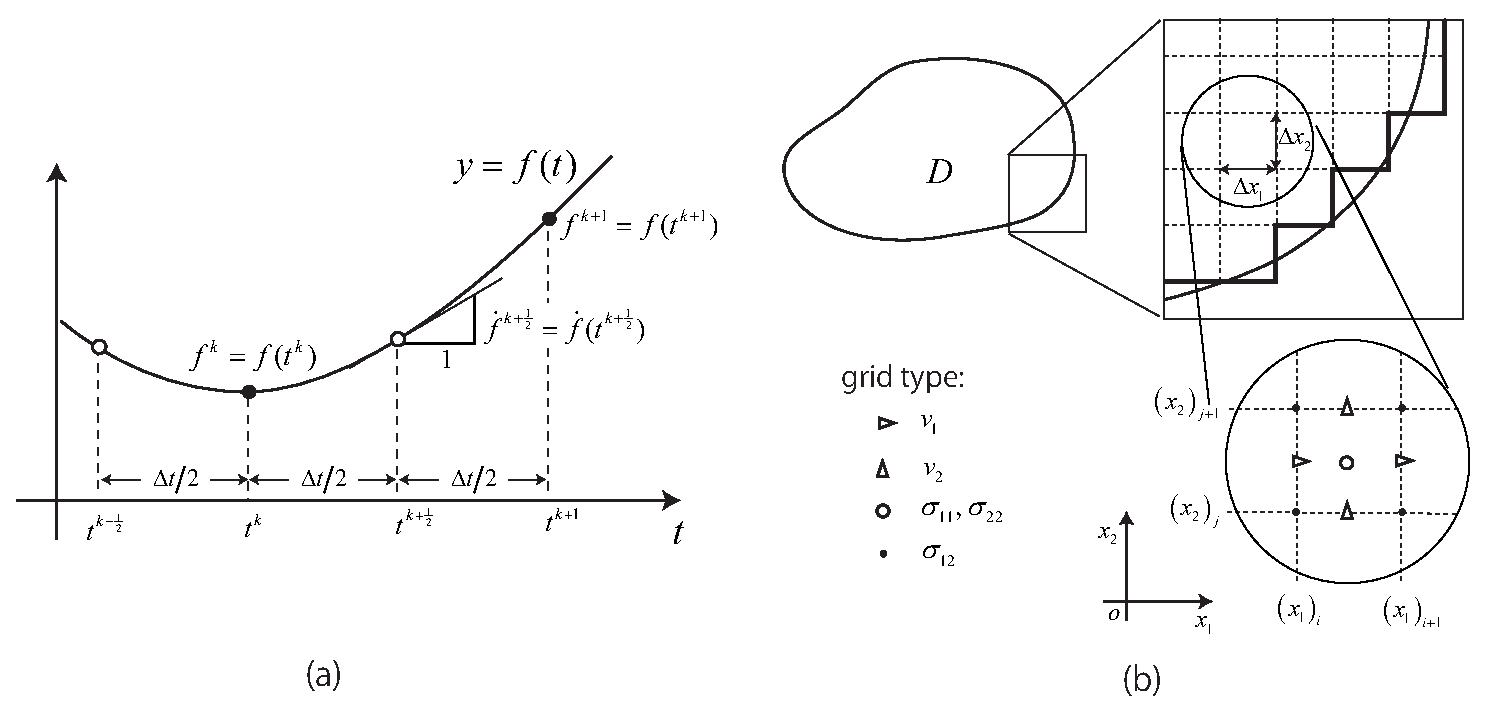
\includegraphics[width=1.0\linewidth]{Figs/FDgrid.eps}
     \end{center}
     \caption{ (a) Finite difference grid arrangement for leap-frog time stepping scheme.
	 (b) The staggered grid system for the central difference approximation 
		of spatial derivatives appearing in the governing elastoynamic 
		equations. A close-up of the unit FD-cell is also shown.
	}
     \label{fig:FDgrids}
\end{figure}
%%%%%%%%%%%%%%%%%%%%%%%%%%%
スタガード格子は図\ref{fig:FDgrids}に示したような,直応力の計算格子を中心にした
$\Delta x_1 \times \Delta x_2$の矩形領域の頂点にせん断応力の,辺上に速度の計算格子を配置したセルを基本単位とする格子配置をとる.これらの格子点における関数値を用いて, 動弾性問題の支配方程式を差分近似すれば,以下のような結果が得られる.
\begin{equation}
	\rho \frac{(v_1)_{i,j+\frac{1}{2}}^{k+1}-(v_1)^k_{i,j+\frac{1}{2}}}{\Delta t}
	=
	\frac{ 
		(\sigma_{11})^{k+\frac{1}{2}}_{i+\frac{1}{2},j+\frac{1}{2}}
		-(\sigma_{11})^{k+\frac{1}{2}}_{i-\frac{1}{2},j+\frac{1}{2}} 
	}
	{\Delta x_1}
	+
	\frac{(\sigma_{12})^{k+\frac{1}{2}}_{i,j+1}-(\sigma_{12})^{k+\frac{1}{2}}_{i,j}}{\Delta x_2}
	\label{eqn:fdtd_v1}
\end{equation}
\begin{equation}
	\rho \frac{(v_2)_{i+\frac{1}{2},j}^{k+1}-(v_2)^k_{i+\frac{1}{2},j}}{\Delta t}
	=
	\frac{(\sigma_{12})^{k+\frac{1}{2}}_{i+1,j}-(\sigma_{12})^{k+\frac{1}{2}}_{i,j}}{\Delta x_1}
	+
	\frac{ 
		(\sigma_{22})^{k+\frac{1}{2}}_{i+\frac{1}{2},j+\frac{1}{2}}
		-(\sigma_{22})^{k+\frac{1}{2}}_{i+\frac{1}{2},j-\frac{1}{2}} 
	}
	{\Delta x_2}
	\label{eqn:fdtd_v2}
\end{equation}
\begin{equation}
	\frac{
		 (\sigma_{11})^{k+\frac{1}{2}}_{i+\frac{1}{2},j+\frac{1}{2}}
		-
		 (\sigma_{11})^{k-\frac{1}{2}}_{i+\frac{1}{2},j+\frac{1}{2}}
	}
	{\Delta t}
	=
	\left( \lambda+2\mu \right)
	\frac{
		(v_1)^{k}_{i+1,j+\frac{1}{2}} - (v_1)^{k}_{i,j+\frac{1}{2}} 
	}
	{\Delta x_1}
	+
	\lambda
	\frac{
		(v_2)^{k}_{i+\frac{1}{2}, j+1} - (v_2)^{k}_{i+\frac{1}{2},j} 
	}
	{\Delta x_2}
	\label{eqn:fdtd_s11}
\end{equation}
\begin{equation}
	\frac{
		 (\sigma_{22})^{k+\frac{1}{2}}_{i+\frac{1}{2},j+\frac{1}{2}}
		-
		 (\sigma_{22})^{k-\frac{1}{2}}_{i+\frac{1}{2},j+\frac{1}{2}}
	}
	{\Delta t}
	=
	\lambda
	\frac{
		(v_1)^{k}_{i+1,j+\frac{1}{2}} - (v_1)^{k}_{i,j+\frac{1}{2}} 
	}
	{\Delta x_1}
	+
	\left( \lambda+2\mu \right)
	\frac{
		(v_2)^{k}_{i+\frac{1}{2}, j+1} - (v_2)^{k}_{i+\frac{1}{2},j} 
	}
	{\Delta x_2}
	\label{eqn:fdtd_s22}
\end{equation}
\begin{equation}
	\frac{
		 (\sigma_{12})^{k+\frac{1}{2}}_{i,j}
		-
		 (\sigma_{12})^{k-\frac{1}{2}}_{i,j}
	}
	{\Delta t}
	=
	\mu \left(
		\frac{
			(v_2)^{k}_{i+\frac{1}{2},j}
			-
			(v_2)^{k}_{i-\frac{1}{2},j}
		}
		{\Delta x_1}
		+
		\frac{
			(v_1)^{k}_{i,j+\frac{1}{2}}
			-
			(v_1)^{k}_{i,j-\frac{1}{2}}
		}
		{\Delta x_2}
	\right)	
	\label{eqn:fdtd_s12}
\end{equation}
以上の式のうち,式(\ref{eqn:fdtd_v1})から(\ref{eqn:fdtd_v2})を,$(v_1)^{k+1}_{i,j+\frac{1}{2}}$や$(v_2)^{k+1}_{i+\frac{1}{2},j}$について解けば, 速度と応力を交替に求める蛙飛び差分スキームによる差分公式が得られる.なお,以上の結果は領域内部にある計算格子において適用可能なものであるため,境界上のグリッドについては,指定された境界条件を反映した差分方程式を用いる必要がある.ここでは,トラクションが与えられた境界における境界条件の与え方について述べる.いま,計算領域を差分セルの集合で近似することを考えると,境界上に配置される可能性のある計算格子は$v_1, v_2$および$\sigma_{12}$である.このうち$\sigma_{12}$については,与えらえた境界値をそのまま代入すればよい.一方,速度$v_1, v_2$については,単位セルサイズが半分になったものと考え,運動方程式を有限体積法の考え方に従って離散化すれば,次のような差分方程式が得られる.
\begin{equation}
	\rho \frac{(v_1)_{i,j+\frac{1}{2}}^{k+1}-(v_1)^k_{i,j+\frac{1}{2}}}{\Delta t}
	=
	\alpha
	\frac{ 
		(\bar\sigma_{11})^{k+\frac{1}{2}}_{i,j+\frac{1}{2}}
		-(\sigma_{11})^{k+\frac{1}{2}}_{i-\frac{\alpha}{2},j+\frac{1}{2}} 
	}
	{\Delta x_1/2}
	+
	\frac{(\bar \sigma_{12})^{k+\frac{1}{2}}_{i,j+1}-(\bar \sigma_{12})^{k+\frac{1}{2}}_{i,j}}{\Delta x_2}
	\label{eqn:fdtd_v1_bnd}
\end{equation}
\begin{equation}
	\rho \frac{(v_2)_{i+\frac{1}{2},j}^{k+1}-(v_2)^k_{i+\frac{1}{2},j}}{\Delta t}
	=
	\frac{(\bar\sigma_{12})^{k+\frac{1}{2}}_{i+1,j}-(\bar\sigma_{12})^{k+\frac{1}{2}}_{i,j}}{\Delta x_1}
	+
	\beta
	\frac{ 
		(\bar \sigma_{22})^{k+\frac{1}{2}}_{i+\frac{1}{2},j}
		-(\sigma_{22})^{k+\frac{1}{2}}_{i+\frac{1}{2},j-\frac{\beta}{2}} 
	}
	{\Delta x_2/2}
	\label{eqn:fdtd_v2_bnd}
\end{equation}
ただし,$\bar{(\cdot)}$は既知の境界値であることを意味し,式(\ref{eqn:fdtd_v1_bnd})と(\ref{eqn:fdtd_v2_bnd})に含まれるパラメータ$\alpha$および$\beta$は,
 \begin{equation}
	\alpha=(n_1)_{i,j+\frac{1}{2}}, \ \ \beta=(n_2)_{i+\frac{1}{2},\, j},
	\label{eqn:def_ab}
\end{equation}
で,外向き法線ベクトル$\fat{n}=(n_1,\, n_2)$の方向により1または-1をとる.以上を用いて,弾性波の2次元伝播散乱解析を行った結果を次節に示す.
%%%%%%%%%%
